\chapter{Literature Review}

In response to the urgent need to reduce carbon emissions and combat climate change, researchers and industry stakeholders have focused on developing and implementing strategies to reduce carbon emissions in maritime shipping.

Figure \ref{publicationRate} shows that the number of publications on energy efficiency and emission reduction in the maritime industry has grown exponentially since 2016. The number of publications from 2006 to 2015 was 76, while from 2016 to 2021, there were 260 publications, indicating a significant increase in interest in decarbonization in the maritime industry.
\autocite{JIMENEZ2022132888}

\begin{figure}[h]
    \centering
    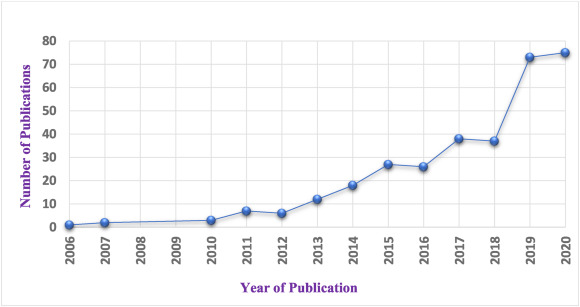
\includegraphics[width=0.7\textwidth]{images/publication_rate.jpg}
    \caption{Number of publications per year in energy efficiency and emission reduction in the maritime domain}
    \label{publicationRate}
\end{figure}

One promising area of research is the use of big data analysis to measure and improve carbon efficiency in maritime shipping. Big data analysis involves the collection and analysis of large and complex data sets to identify patterns, trends, and insights. In the context of maritime shipping, big data analysis can be used to measure carbon emissions and identify opportunities for improvement.

The purpose of this literatsure review is to examine the current state of research on carbon emissions in maritime shipping, with a focus on the Energy The Energy Efficiency eXisting ship Index (EEXI) and Carbon Intensity Indicator (CII) as key metrics for measuring carbon efficiency. The review will provide an overview of the current state of research on these metrics, their strengths and limitations, and their relevance for the maritime shipping industry.

The review will begin by exploring the importance of reducing carbon emissions in maritime shipping and the regulatory and policy frameworks that have been established to address this issue. It will then provide an overview of the EEXI and CII metrics, including their definitions, methodologies for calculating them, and their role in measuring carbon efficiency.

The literature review will also examine the current research on the relationship between EEXI, CII, and carbon emissions in maritime shipping, with a particular focus on the use of big data analysis to measure and improve carbon efficiency. It will explore the potential for big data analysis to provide more accurate and comprehensive data on carbon emissions, and to identify opportunities for operational and technological improvements.

Overall, this literature review will provide a comprehensive overview of the current state of research on carbon emissions in maritime shipping, with a focus on the EEXI and CII metrics and the potential for big data analysis to guide and inform strategies for improving carbon efficiency in the industry.


\section{Litrature Review}


Review by \citeauthor{en15217910} \autocite{en15217910} shows that Maritime shipping is a crucial aspect of global trade and the global economy, with over 85\% of the volume of global trade in goods transported by sea.
However, maritime transport also has significant environmental impacts, including carbon emissions.
Approximately 3.3\% of the world's carbon dioxide (CO2) emissions are attributable to maritime transport, with emissions from marine diesel oil (MDO), marine fuel oil (MFO), and heavy fuel oil (HFO) all contributing to the problem.
Reducing carbon emissions in the maritime shipping industry is a significant challenge, but there are a range of strategies that can be used to achieve this goal.
Alternative fuels, energy efficiency improvements, and operational measures all have the potential to reduce emissions, but they also have significant economic and resource constraints.


Paper by \citeauthor{en15176150} \autocite{en15176150} mentions that  Despite its significant contribution to global economic growth, maritime transport also generates negative externalities, primarily in the form of greenhouse gas (GHG) emissions.
They discus how digitalization and the use of artificial intelligence (AI) are being explored as potential ways to reduce emissions in maritime shipping.
AI algorithms can optimize shipping routes, reduce fuel consumption, and minimize emissions. Additionally, digitalization can enable better data collection and analysis, which can facilitate more accurate emissions reporting and monitoring.

According to \citeauthor{jmse10020129} \autocite{jmse10020129}, the use of automatic identification system (AIS) to estimate ship emissions, which is an advantage due to the system's ability to provide real-time navigational information.
Studies have been conducted utilizing AIS data to estimate ship emissions in different regions, such as Hong Kong and the Pearl River Delta, Las Palmas Port, Qingdao Port, Tianjin port, Naples port, and unidentified vessels with missing ship parameters.
The studies have focused on macro-scale spatial and temporal resolution, high-resolution ship emission inventory, high temporal-spatial ship emission inventory, higher spatial-temporal resolution, and real-time ship emission monitoring.
It proposes simulation model based on AIS data, specification and what-if scenarios as shown in Figure \ref{simaulationFramework}

\begin{figure}[h]
    \centering
    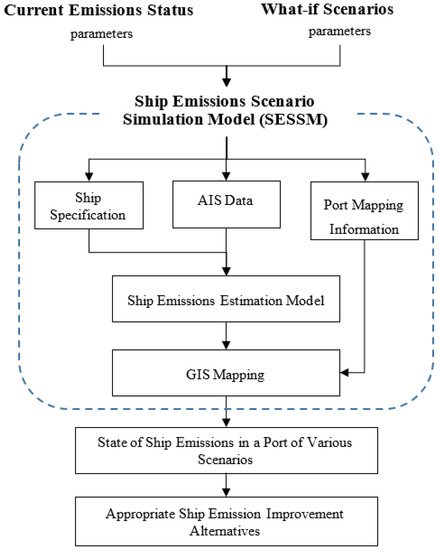
\includegraphics[width=0.5\textwidth]{images/simulation_framework.jpeg}
    \caption{Simulation framework}
    \label{simaulationFramework}
\end{figure}


Research by \citeauthor{SOU2022113239} \autocite{SOU2022113239}, discusses the need for carbon intensity indicators (CIIs) as performance monitoring tools in the shipping industry, particularly for tracking energy efficiency trends and progress towards climate targets.
The review highlights the lack of consensus on suitable CIIs, as proposed by various countries to the International Maritime Organization (IMO), and the need for a more comprehensive understanding of global progress towards carbon intensity targets from both demand and supply side indicators.
The study aims to address this issue by analyzing CIIs for shipping and the factors that influence the carbon intensity of shipping at the global level. Index decomposition analysis (IDA) is used to quantify the contribution of various factors, including energy efficiency, to changes in carbon intensity from 2012 to 2018.



According to report by \citeauthor{stevenson_2021_bulker} \autocite{stevenson_2021_bulker}, The International Maritime Organization will introduce Energy Efficiency eXisting ship Index (EEXI) and Carbon Intensity Indicator (CII) regulations in 2023 as part of the wider decarbonisation goals for shipping. More than three-quarters of the existing fleet will not initially meet EEXI baselines and will need to take action to achieve compliance, with overridable engine power limitations (oEPL) expected to be a popular option. However, the effect on vessel operations over a year will be quite small due to the relatively small number of hours where steaming speeds would exceed oEPL limits. The compliance with EEXI can result in modest improvements in AER, CII, and annual CO\textsubscript{2}. emissions.

\begin{figure}[h]
    \centering
    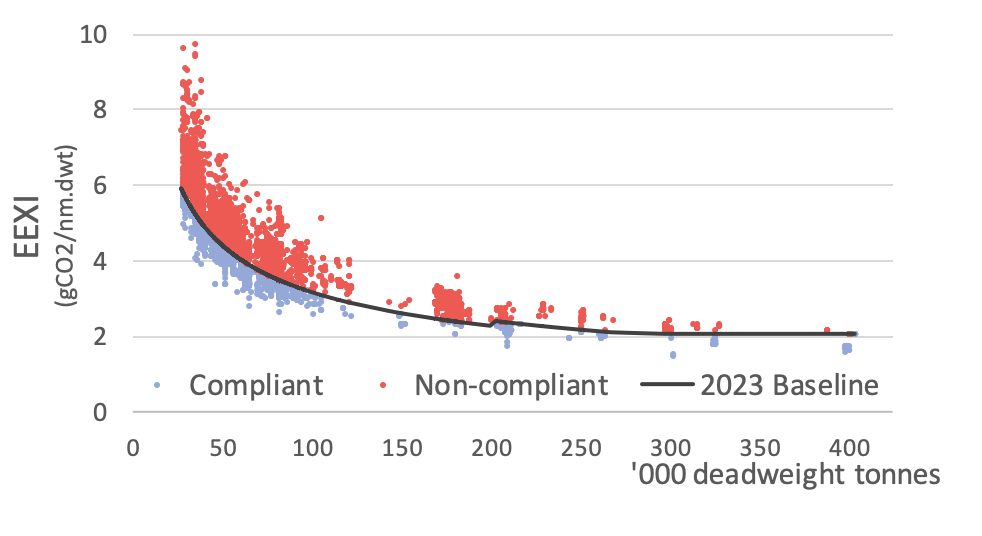
\includegraphics[width=0.7\textwidth]{images/eexi_non_compliant.png}
    \caption{EEXI BULKER ESTIMATES VS. 2023 BASELINE}
    \label{eexiNonCompliant}
\end{figure}


The International Maritime Organization (IMO) has made maritime decarbonization a priority, setting targets to reduce greenhouse gas emissions from ships.
To achieve these targets, the IMO has adopted mandatory measures, including the carbon intensity indicator (CII), which measures carbon emissions per unit transport work for each ship.
But \citeauthor{WANG2021100005} \autocite{WANG2021100005} argues there are potential paradoxes with the CII, as it may increase carbon emissions in some situations.
There are at least four potential versions of the CII, including supply-based, demand-based, distance-based, and sailing time-based, but the IMO has not yet agreed on which to use.
More elaborate models and indicators should be developed to analyze the potential impacts of the CII and achieve utmost carbon emissions reduction.

In \citetitle{doi:10.1080/03088839.2020.1788731} \autocite{doi:10.1080/03088839.2020.1788731}, author \citeauthor{doi:10.1080/03088839.2020.1788731} explains how Big data and artificial intelligence (AI) have become essential components of data-driven decision-making in most industries.
However, the maritime industry still relies on intuition more than on data, mainly because of the vast size of its network and planning problems.
The maritime industry generates large amounts of data that, if appropriately utilised in decision-making, can improve maritime safety, reduce environmental impacts, and minimise cost. In this review, we focus on studies that deal with big data and AI applications within the maritime context to map the conceptual structure of the field and identify future research avenues.
AIS data to investigate the impact of speed reduction on fuel consumption and carbon emissions in the shipping industry.
The study found that a 10\% reduction in ship speed could result in a 17\% reduction in fuel consumption and a corresponding reduction in carbon emissions.
The authors suggested that reducing ship speed is an effective way to reduce fuel consumption and carbon emissions in the maritime industry.

\begin{figure}[h]
    \centering
    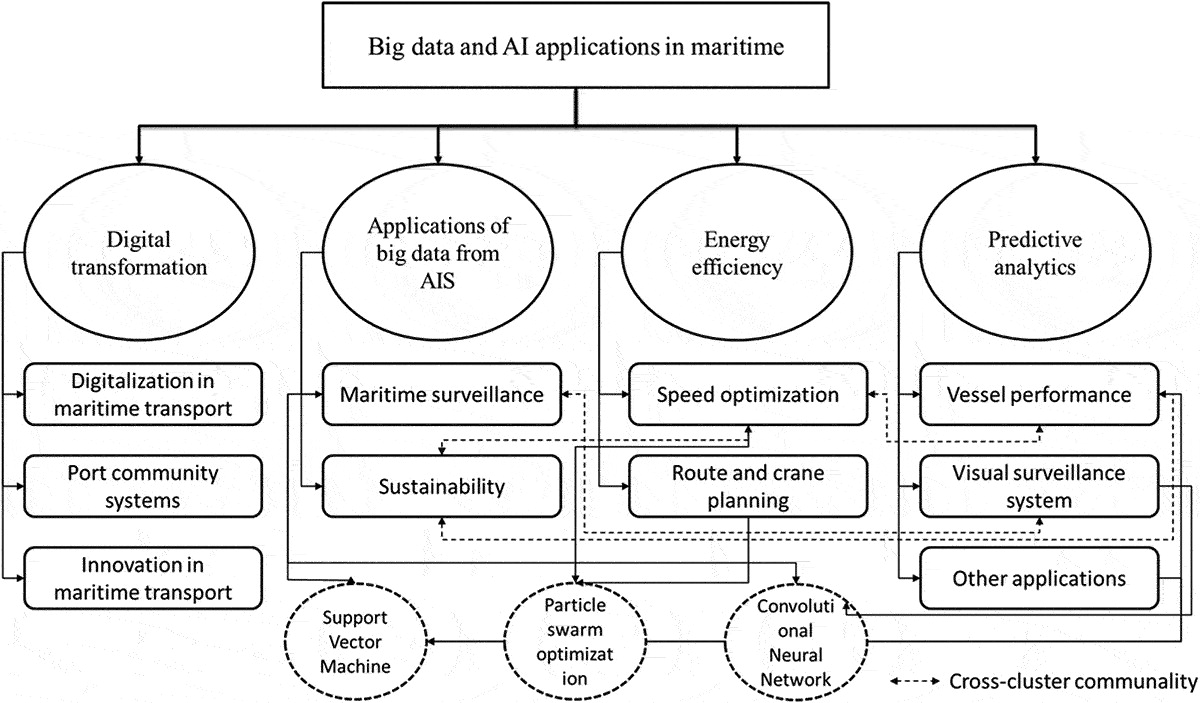
\includegraphics[width=0.7\textwidth]{images/application_big_data_martime.jpeg}
    \caption{Application of Big dada and AI in maritime industry}
    \label{applicationBigDataMartime}
\end{figure}

The study by \citeauthor{acomi2014improving} \autocite{acomi2014improving}, delves into the realm of maritime environmental conservation, emphasizing the Energy Efficiency Operational Index (EEOI) as a pivotal tool.
Addressing concerns of marine pollution encompassing water and air aspects, the paper underscores international efforts for emission reduction in shipping.
The EEOI, designed to measure carbon emissions per unit of transport work, aids ship-owners and operators in enhancing energy efficiency during operational voyages.
The research demonstrates how commercial software and a custom-developed program estimate EEOI values pre-voyage and onboard, revealing the influence of unpredictable factors on energy efficiency.
This analysis not only showcases the EEOI's significance in curbing emissions but also highlights its vital role in the broader context of maritime sustainability and environmental protection.

\subsection{Conclusion}

In this section, we have reviewed the literature on carbon emissions in maritime shipping, with a focus on the EEOI and CII metrics and the potential for big data analysis to guide and inform strategies for improving carbon efficiency in the industry.

In conclusion, the literature reviewed emphasizes the importance of addressing the significant environmental impact of carbon emissions in the maritime shipping industry.
While there are various strategies to reduce emissions, such as alternative fuels, energy efficiency improvements, and operational measures, they have significant economic and resource constraints.
Digitalization and the use of artificial intelligence (AI) are being explored as potential ways to reduce emissions by optimizing shipping routes, reducing fuel consumption, and minimizing emissions.
Furthermore, the use of automatic identification system (AIS) data can facilitate real-time emissions monitoring, while carbon intensity indicators (CIIs) can be used as performance monitoring tools.
The International Maritime Organization (IMO) has made maritime decarbonization a priority by setting targets to reduce greenhouse gas emissions from ships and introducing regulations like EEXI and CII.
However, potential paradoxes with the CII and lack of consensus on suitable CIIs highlight the need for more elaborate models and indicators to achieve utmost carbon emissions reduction. Big data and AI applications have the potential to improve maritime safety, reduce environmental impacts, and minimize costs.
Overall, more research is needed to address the challenges of monitoring and reducing carbon emissions in the maritime shipping industry while meeting global trade demands.
